\documentclass[10pt]{seminar} 

\renewcommand{\baselinestretch}{1}

\usepackage{amsmath}

\renewcommand{\printlandscape}{\special{landscape}}

\usepackage{ulem}



\input{seminar.bug}

%\usepackage{fancybox}

\usepackage{epsfig}

%\usepackage{times}


\usepackage{amssymb}

\usepackage{amscd}

\usepackage{graphics}

\usepackage{pstricks}

%\usepackage{chicago}

%\usepackage{fullpage}

\slideframe{none}

\begin{document}

\newtheorem{proposition}{Proposition}

\newtheorem{definition}{Definition}

\newtheorem{corollary}{Corollary}

\newtheorem{theorem}{Theorem}

\newtheorem{lemma}{Lemma}

\def\argmax{\mathop{\rm argmax}\limits}  


%\slideframe{Oval}

\sffamily 


\begin{slide}
\begin{center}

Multivariate Calculus  \end{center}
 
 \newslide
 \small 
 For our last two classes we'll deal with functions of more than one variable
 
\ \\ Ex: A person's utility is a function of apples ($x$) and bananas $(y)$, and looks like $$U(x, y)=(5+x)^{1\over 2}+(2y+1)^{1\over 2}+xy$$

\begin{center}
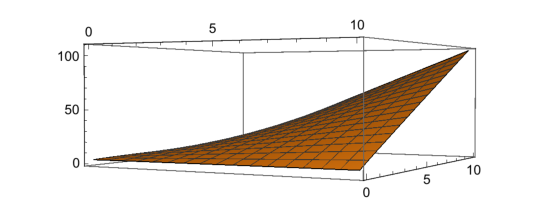
\epsfig{file=3D.eps, scale=1}
\end{center}
 
 \ \\We want to see how $U$ changes as $x$ and $y$ change
 
 \newslide
 First, we'll consider what happens to utility as $x$ changes and $y$ remains fixed (we will treat $y$ as a constant)
 
 \ \\${{\partial f}\over {\partial x}}$ is the \textit{partial derivative} of $f$ with respect to $x$ (with ${{\partial f}\over {\partial y}}$ defined similarly)
 
$$\begin{array}{rcl}U(x, y)&=&(5+x)^{1\over 2}+(2y+1)^{1\over 2}+xy \vspace{.2in} \\

 \vspace{.2in}
 
{{\partial U}\over{\partial x}} &=& y+{1\over 2}(5+x)^{-{1\over 2}}\\

  \vspace{.2in}
  
{{\partial U}\over{\partial y}} &=& x+{1\over 2}(2y+1)^{-{1\over 2}}*2\\
&=& x+(2y+1)^{-{1\over 2}}
\end{array}$$

\newslide
$$U(x, y)=(5+x)^{1\over 2}+(2y+1)^{1\over 2}+xy $$

$${{\partial U}\over{\partial x}} = y+{1\over 2}(5+x)^{-{1\over 2}}$$
\begin{center}
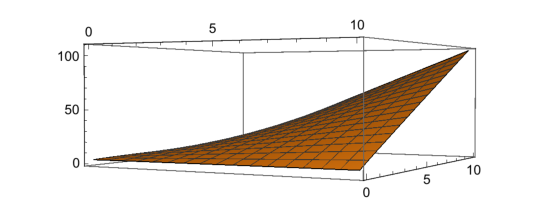
\epsfig{file=3D.eps, scale=.7}
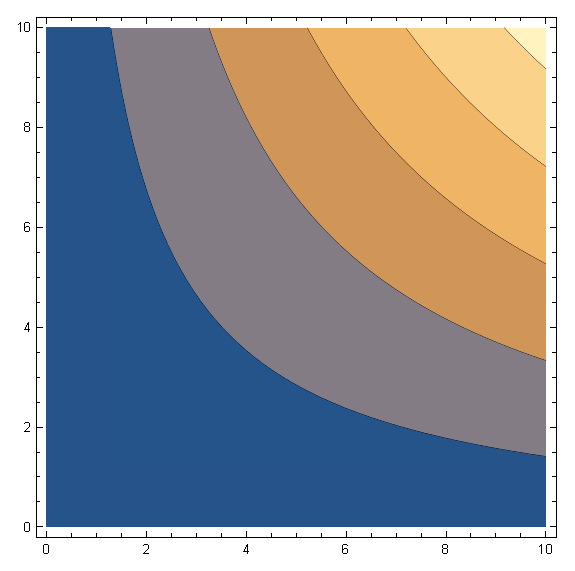
\epsfig{file=contour.eps, scale=.4} 
\epsfig{file=legend.eps, scale=.4}
\end{center}
%Contour plot, isoquant for production functions, indifference curve for utilities
\begin{itemize}


\item ${{\partial U}\over{\partial x}}$ always positive
\item ${{\partial U}\over{\partial x}}$ greater for greater $y$
\item ${{\partial U}\over{\partial x}}$ smaller for greater $x$
\end{itemize}

\newslide

\begin{center}
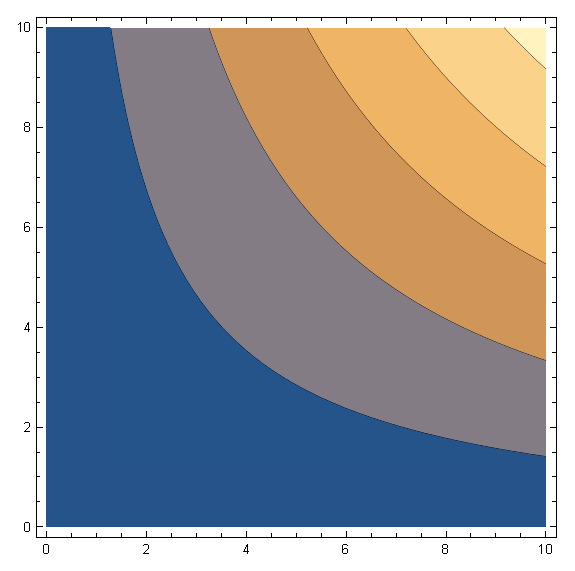
\epsfig{file=contour.eps, scale=.4} 
\epsfig{file=legend.eps, scale=.4}
\end{center}
%Contour plot, isoquant for production functions, indifference curve for utilities
\begin{itemize}

\item ${{\partial U}\over{\partial x}}$ always positive: utility is always increasing in $x$
\item ${{\partial U}\over{\partial x}}$ increasing in $y$: the goods are \textit{complements} in the sense that an increase in $y$ raises the marginal value of $x$
\item ${{\partial U}\over{\partial x}}$ decreasing in $x$: $x$ exhibits diminishing marginal utility
\end{itemize}

\newslide

The rules of partial differentiation are identical to the rules of regular differentiation, treating all other variables as constants

\ \\Example: Let $$U(w, x, y, z)=10wxz+x^3-wy+y^{1\over 2}-z^{10}+zw$$ Then:

$$\begin{array}{rcl}

{{\partial U}\over{\partial w}} & = & 10xz-y+z \vspace{.1in}\\

\vspace{.1in}

{{\partial U}\over{\partial x}} & = & 10wz+3x^2\\

\vspace{.1in}

{{\partial U}\over{\partial y}} & = & -w+{1\over 2}y^{-{1\over 2}}\\

\vspace{.1in}

{{\partial U}\over{\partial z}} & = & 10wx-10z^9+w\\



\end{array}
$$

\newslide
Second derivatives

\ \\The \textit{second partial derivative} of $f$ with respect to any variable $x$ is written $${{\partial^2 f}\over{\partial x^2}}={{\partial}\over{\partial x}} {{\partial f}\over{\partial x}}  $$ 

\ \\The \textit{mixed partial derivatives } (or \textit{cross partial derivatives}) of $f(x, y)$ are written $$ {{\partial^2 f}\over{\partial x \partial y}}= {{\partial}\over{\partial x}} {{\partial f}\over{\partial y}} $$

\newslide
Example:

$$U(w, x, y, z)=10wxz+x^3-wy+y^{1\over 2}-z^{10}+zw$$ 

$$\begin{array}{rcl}
{{\partial U}\over{\partial x}} & = & 10wz+3x^2\\
{{\partial^2 U}\over{\partial x^2}} &=& 6x\\
 {{\partial^2 U}\over{\partial x \partial w}} &=&10z \\
  {{\partial^2 U}\over{\partial x \partial y}} &=& 0\\
  {{\partial^2 U}\over{\partial x \partial z}} &=& 10w\\

&&\hbox{etc...} 
\end{array}
$$

\newslide

Notation

\ \\There are many different ways to denote a partial derivative; the following are equivalent:
$${{\partial f}\over{\partial x}} \hspace{.15in} {{\partial }\over{\partial x}} f \hspace{.15in} f_1 \hbox{ (provided $x$ is the first argument of $f$) } \hspace{.15in} f_x \hspace{.15in} D_x f$$

\ \\Similarly for cross partials the following are equivalent:

$${{\partial^2 f}\over{\partial xy}} \hspace{.15in} {{\partial }\over{\partial x}} {{\partial f}\over {\partial y}} \hspace{.15in} f_{12}  \hspace{.15in} f_{xy} \hspace{.15in} D_{xy} f$$


\newslide

The mixed derivative theorem

\ \\If $f$ has continuous first, second and mixed partial derivatives (as in these derivatives exist and are themselves continuous), then $f$ is a class $C^2$ function

\ \\A class $C^k$ function is defined similarly, with $k$ representing the number of partial derivatives $f$ has that exist and are continuous (i.e. $ {{\partial^k f}\over{\partial x_1...}}$)

\ \\Your book calls a class $C^2$ function \textit{smooth}

\ \\Theorem: If $f$ is a smooth function then $f_{xy}=f_{yx}$ for all $x, y$

\newslide

Example:

$$U(w, x, y, z)=10wxz+x^3-wy+y^{1\over 2}-z^{10}+zw$$ 

$$\begin{array}{rcl}
{{\partial U}\over{\partial x}} & = & 10wz+3x^2\\
{{\partial U}\over{\partial y}} &=& -w+{1\over 2}y^{-{1\over 2}}\\
 {{\partial U}\over{\partial z}} &=&10wx-10z^9+w \\
  {{\partial^2 U}\over{\partial x \partial y}} &=& 0\\
  {{\partial^2 U}\over{\partial y \partial x}} &=&0\\
    {{\partial^2 U}\over{\partial x \partial z}} &=& 10w\\
    {{\partial^2 U}\over{\partial z \partial x}} &=& 10w\\
&&\hbox{etc...} 
\end{array}
$$

\newslide

The chain rule for two variables

\ \\Let $z=f(x, y)$ be a smooth function and suppose that $x$ and $y$ are themselves functions of a third variable, $t$

\ \\$$x=g(t) \hbox{ and }y=h(t)$$ Then $$z=F(t)=f(g(t),h(t))$$

\ \\The \textit{chain rule} says that $$F^\prime(t)=f_1(g(t), h(t))g^\prime(t)+f_2(g(t), h(t))h^\prime(t)$$ or alternatively, 

$${{dz}\over {dt}}={{\partial f}\over {\partial x}}{{dx}\over {dt}}+{{\partial f}\over {\partial y}}{{dy}\over {dt}}$$


\newslide
$${{dz}\over {dt}}={{\partial f}\over {\partial x}}{{dx}\over {dt}}+{{\partial f}\over {\partial y}}{{dy}\over {dt}}$$

\ \\Intuition: As $t$ changes by a small amount, the overall change in $z$ is the sum of the indirect effects of $t$'s change on $x$ and $y$

\ \\Example: Let $$f(x, y)=xy^4+x^3y^2 \hbox{ and }x=2-3t\hbox{ and }y=4+5t$$

\ \\To find $f^\prime(t)$ we could reexpress $f$ in terms of $t$ by substituting $x(t)$ and $y(t)$ back into $f$; OR we could use the chain rule letting $z(t)=f(x, y)$

\newslide

$$f(x, y)=xy^4+x^3y^2 \hbox{ and }x=2-3t\hbox{ and }y=4+5t$$

$$
\begin{array}{rcl}
{{dz}\over{dt}} &=& {{\partial f}\over {\partial x}}{{dx}\over {dt}}+{{\partial f}\over {\partial y}}{{dy}\over {dt}}\\
&=& (y^4 +3x^2y^2){{dx}\over {dt}}+(4xy^3+2x^3y){{dy}\over {dt}}\\
{{dx}\over {dt}}&=&-3 \\
{{dy}\over {dt}}&=& 5  \vspace{.1in} \\

{{dz}\over{dt}}  &=& -3(y^4 +3x^2y^2)+5(4xy^3+2x^3y)
\end{array}
$$



You can convince yourself this is true by differentiating $$(2-3t)(4+5t)^4+(2-3t)^3(4+5t)^2 $$ with respect to $t$ and seeing if it equals $$-3((4+5t)^4 +3(2-3t)^2(4+5t)^2)+5(4(2-3t)(4+5t)^3+2(2-3t)^3(4+5t))!$$

\newslide

Total derivatives

\ \\Suppose that $y=h(x)$ and $z=F(x)=f(x, y)$; then $F^\prime(x)$ is the \textit{total derivative} of $z$ with respect to $x$

\ \\This is different from ${{\partial f}\over{\partial x}}$, which treats $y$ as a constant; the total derivative accounts for the fact that a change in $x$ causes both its own (direct) change in $z$, and also an indirect change in $z$ through its effect on $y$

\ \\Using the chain rule we get that $${{dz}\over{dx}}=f_x {{dx}\over{dx}}+f_y{{ dy}\over{ dx}}$$

$${{dz}\over{dx}}=\underbrace{f_x}_{\hbox{Direct effect of $x$ on $f$} }+\underbrace{f_y dy/dx}_{\hbox{Indirect effect of $x$ on $f$ via $y$}} $$
\newslide

Suppose that $f(x_1, x_2, ..., x_k)$ is a smooth function of $k$ variables, where each $x_k$ is itself a function of some other variable, $t$

$$f(x_1, x_2, ..., x_k) =F(t)$$
The chain rule says that $${{dF}\over{ dt}}=\sum_{i=1}^k {{\partial f}\over{\partial x_i}}{{ dx_i}\over{ dt}}$$
Now suppose that each $x_k$ is a function of \textit{several} other variables, $t, u, ...$

$$f(x_1, x_2, ..., x_k) =F(t, u, ...)$$
The chain rule says that $${{\partial F}\over{\partial t}}=\sum_{i=1}^k {{\partial f}\over{\partial x_i}}{{\partial x_i}\over{\partial t}}$$


\newslide

The gradient

\ \\Let $f(x_1, x_2, ..., x_k) $ be a function of $k$ variables; at each point $(x_1, x_2, ..., x_k)$ we define the gradient vector $D f(x_1, ..., x_k)$ as follows:

$$D f(x_1, ..., x_k)= \nabla f (x_1, ..., x_k)= \begin{bmatrix}f_{x_1}(x_1, x_2, ..., x_k) \\
f_{x_2}(x_1, x_2, ..., x_k) \\
...\\
f_{x_k}(x_1, x_2, ..., x_k) 
\end{bmatrix}$$

\ \\It's the vector whose components are the $k$ partial derivatives of $f$


\newslide
$\nabla f(\mathbf{x})$ points in the direction of the greatest rate of increase of $f$ evaluated at $\mathbf{x}$; its magnitude is the slope of $f$ in that direction

\ \\Example: $$U(x, y)=-(x-5)^2-(y-5)^2$$

\begin{center}
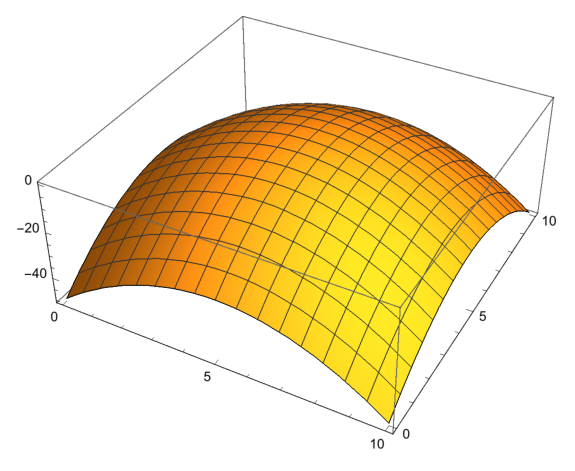
\epsfig{file=quadratic.eps, scale=.7}
\end{center}

\newslide

\begin{center}
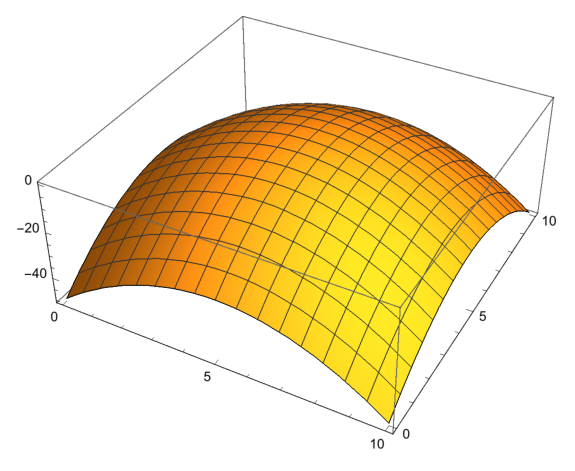
\epsfig{file=quadratic.eps, scale=.45}
\end{center}

$$\begin{array}{lcl}
\nabla U(x, y)&=&(10-2x, 10-2y)\\
\nabla U(0, 0)&=&(10, 10)\\
\nabla U(2, 2)&=&(6, 6)\\
\nabla U(0, 5)&=&(10, 0)\\
\nabla U(0, 2.5)&=&(10, 5)\end{array}$$

\newslide
The Hessian matrix

\ \\A matrix that consists of all of the cross-partial derivatives of $f(x_1, x_2, ..., x_k) = f(\mathbf{x})$ in the following way:

$$D^2f(\mathbf{x})= \begin{bmatrix}
f_{x_1x_1}(\mathbf{x})& f_{x_1x_2}(\mathbf{x})& ...& f_{x_1x_k}(\mathbf{x})\\
f_{x_2x_1}(\mathbf{x})& f_{x_2x_2}(\mathbf{x})& ...& f_{x_2x_k}(\mathbf{x})\\
...&...&...&\\

f_{x_kx_1}(\mathbf{x})& f_{x_kx_2}(\mathbf{x})& ...& f_{x_kx_k}(\mathbf{x})\\


\end{bmatrix}$$

This matrix is square and symmetric (why?)

\newslide
Example

 $$U(x, y)=-(x-5)^2-(y-5)^2$$
 
$$ \nabla U(x, y)=(10-2x, 10-2y)$$

$$D^2 f(\mathbf{x}) =\begin{bmatrix}
-2 & 0\\ 0& -2
\end{bmatrix}$$

\newslide

Critical points and their classification

\ \\For a function of many variables, $f(x_1, x_2, ..., x_k)=f(\mathbf{x})$,  critical points $\mathbf{x}$ are defined as points where the gradient vector $\nabla f(\mathbf{x})$ equals zero

\ \\As with functions of one variable, we use second-order conditions to determine what kind of critical point we have:

\begin{itemize}
\item[1] If $f$ has a local maximum at $\mathbf{x}^*$ then $\nabla f(\mathbf{x}^*)=\mathbf{0}$ and $D^2f(\mathbf{x}^*)$ is negative semidefinite
\item[2]  If $\nabla f(\mathbf{x}^*)=\mathbf{0}$ and $D^2f(\mathbf{x}^*)$ is negative definite then $f$ has a local maximum at $\mathbf{x}^*$ 
\item[1'] If $f$ has a local minimum at $\mathbf{x}^*$ then $\nabla f(\mathbf{x}^*)=\mathbf{0}$ and $D^2f(\mathbf{x}^*)$ is positive semidefinite
\item[2'] If $\nabla f(\mathbf{x}^*)=\mathbf{0}$ and $D^2f(\mathbf{x}^*)$ is positive definite then $f$ has a local minimum at $\mathbf{x}^*$ 
\end{itemize}

\newslide
Example

 $$U(x, y)=-(x-5)^2-(y-5)^2$$
 
$$ \nabla U(x, y)=(10-2x, 10-2y)$$

$$D^2 f(\mathbf{x}) =\begin{bmatrix}
-2 & 0\\ 0& -2
\end{bmatrix}$$

\ \\The Hessian is negative definite for all $\mathbf{x}$ because the determinant is always strictly positive and both diagonal entries are strictly negative

\ \\Critical point $\mathbf{x}=(x, y)=(5,5)$ is a local maximum

\newslide

Global optima

\ \\Knowing that $\mathbf{x}$ is a local maximum doesn't help us if we are looking for a global maximum; if $f$ is concave or convex then we know a lot more

\ \\$f:\mathbb{R}^n\rightarrow \mathbb{R}$ is \textit{concave} if and only if for any $\mathbf{x_1, x_2}\in \mathbb{R}^n$ and any $\alpha\in [0, 1]$: $$f(\alpha \mathbf{x_1}+(1-\alpha)\mathbf{x_2})\geq \alpha f(\mathbf{x_1})+(1-\alpha)f(\mathbf{x_2})$$

\begin{itemize}
\item The function $f(\mathbf{x})$ is concave (convex) if and only if the Hessian $D^2f(\mathbf{x})$ is negative (positive) semidefinite FOR ALL $\mathbf{x}$
\item The concave (convex) function $f(\mathbf{x})$ attains a global maximum (minimum) at $\mathbf{x}^*$ if and only if the gradient $\nabla f(\mathbf{x}^*)=\mathbf{0}$
\end{itemize}

$\Rightarrow$ Every critical point of a concave function is a global maximum\\
$\Rightarrow$ Every critical point of a convex function is a global minimum

\newslide

\small
Concavity / convexity is tremendously helpful in classifying critical points; the following are tricks that can be used to help determine whether a function is concave / convex:

\begin{itemize}
\item The sum of two concave functions is concave; the sum of two convex functions is convex
\item A concave function of one variable is a concave function of many variables: if $f(x_1, x_2, ..., x_k)=g(x_1)$ with $g$ concave, then $f$ is concave
\item $f$ is concave if and only if $-f$ is convex
\item A \textit{strictly} concave function has at most one global maximum
\item Let $g$ be a nondecreasing and concave function of one variable; then if $f(\mathbf{x})$ is concave so is $g(f(\mathbf{x}))$
\item Let $h$ be a nondecreasing and convex function of one variable; then if $f(\mathbf{x})$ is convex so is $h(f(\mathbf{x}))$
\end{itemize}

\newslide
Example: Let $$U(x, y)= -(x-2)(y+5)$$

\ \\Find the critical points of $U$

\ \\Can you classify the critical point(s)?

\newslide

$$U(x, y)= -(x-2)(y+5)$$

Critical point: $(2, -5)$

$$D^2 U=
\begin{bmatrix}
0& -1\\
-1& 0
\end{bmatrix}
$$

\ \\Det$[D^2 U]=-1<0$, and so the critical point is a saddle point

\ \\ \begin{center}
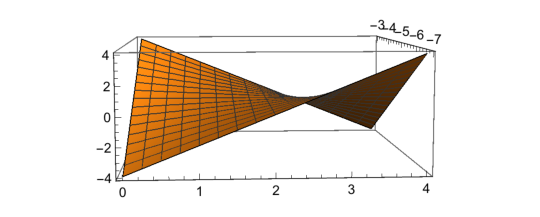
\epsfig{file=saddle.eps}
\end{center}

\newslide
Example: Let $$U(x, y)= -x^2+4xy-4y^2$$

\ \\Find the critical points of $U$

\ \\Can you classify the critical point(s)?

\newslide
$$U(x, y)= -x^2+4xy-4y^2$$
An infinite number of critical points:  $(2C, C)$ for all $C\in \mathbb{R}$

$$D^2 U=
\begin{bmatrix}
-2& 4\\
4& -8
\end{bmatrix}
$$
Det$[D^2 U]=0$, and all diagonals are negative, so Hessian is negative semidefinite for all $\mathbf{x}$ and $U$ is concave: all critical points are global optima
 \begin{center}
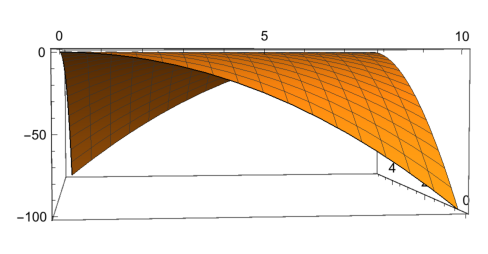
\epsfig{file=manyOpt.eps, scale=.8}
\end{center}


 \end{slide}
 
 \end{document}








